\documentclass[12pt]{jreport}
\usepackage{comment}
\usepackage{./sty/eclepsf}
\usepackage{tascmac}
\usepackage{tabularx}
\usepackage{listliketab}
\usepackage[longnamesfirst]{natbib}
\usepackage[dvipdfmx]{graphics}
\usepackage[dvipdfmx]{graphicx}
\usepackage[dvipdfmx]{color}
\usepackage{subfigure}
\usepackage{alltt}
\usepackage{here}
\usepackage{afterpage}
\usepackage{./sty/ncodeline}
%\usepackage[dvipdfmx, colorlinks, breaklinks,%
\usepackage[dvipdfmx, breaklinks,%
bookmarks=true, bookmarksnumbered=true,%
bookmarkstype=toc, bookmarksopen=true,bookmarksopenlevel=3,%
pdftitle={WatanabeSatoki Master's thesis},%
]{hyperref}
\usepackage{bookmark}

\AtBeginDvi{\special{pdf:tounicode EUC-UCS2}}

\usepackage{fancyhdr}

\usepackage{./sty/doxygenorig}

\usepackage{indentfirst}
\usepackage{url}
\usepackage{listings,./sty/jlisting}

\def\lstlistingname{プログラム}

\lstset{%
 language={C++},
 %backgroundcolor={\color[gray]{.85}},%
 basicstyle={\small\ttfamily},%
 identifierstyle={\small},%
 commentstyle={\small\itshape},%
 keywordstyle={\small\bfseries},%
 ndkeywordstyle={\small\ttfamily},%
 stringstyle={\small\ttfamily},
 frame={tb},
 framesep=1zw,
 breaklines=true,
 numbers=left,%
 xrightmargin=0zw,%
 xleftmargin=1.5zw,%
 numberstyle={\scriptsize},%
 stepnumber=1,
 numbersep=1zw,%
 lineskip=-0.5ex%
}

\usepackage{amssymb}
%\usepackage{supertabular,multirow}

\usepackage{array}
\newcolumntype{M}[1]{>{\centering\arraybackslash}m{#1}}

% A4  size: 297mm*210mm %1pt = 0.35mm
\setlength{\topmargin}{-3.4mm} % 10pt 25.4mm - 3.4mm = 22mm
\setlength{\oddsidemargin}{-0.4mm} % 25.4mm - 0.4mm = 25mm
\setlength{\evensidemargin}{-0.4mm} % 25.4mm - 0.4mm = 25mm
\setlength{\textheight}{231mm} % 660pt % original is 225.75mm 645pt
\setlength{\textwidth}{160mm} % 457pt

\renewcommand{\topfraction}{.99}
\renewcommand{\textfraction}{.0}
\renewcommand{\floatpagefraction}{.99}
\renewcommand{\bibname}{参考文献}


\pagestyle{fancy}
\lhead[]{}

\makeatletter
\def\chaptermark#1{\markboth {\ifnum \c@secnumdepth>\m@ne
\@chapapp\ \thechapter \@chappos\ \fi #1}{}}
\makeatother

% タイトル
\def\title{個別文脈依存蓄積差分確認方式による利用規約読解時間の短縮}
% 英語タイトル
\def\etitle{Reduction of reading time of Terms of Service by individual context-dependent accumulated difference confirmation method}
% 著者(日本語)
\def\author{渡邉 聡紀}
% 著者(英語)
\def\eauthor{Watanabe Satoki}
% 学部・研究科
\def\dept{慶應義塾大学大学院 政策・メディア研究科}
% 学部・研究科(英語)
\def\edept{Keio University Graduate School of Media and Governance}

\begin{document}

\pagenumbering{roman}
\begin{titlepage}
  \begin{center}
    \begin{large}
      修士論文   2022年度(令和4年度)\\
      \vspace{24pt}
      \title
      \end{large}
  \end{center}
  \vspace{40em}
  \begin{flushright}
    \large \dept\\
    \author
  \end{flushright}
\end{titlepage}

\thispagestyle{empty}


修士論文要旨 - 2022年度 (令和4年度)
\begin{center}
\begin{large}
\begin{tabular}{|M{0.97\linewidth}|}
    \hline
      \title \\
    \hline
\end{tabular}
\end{large}
\end{center}

~ \\

インターネット利用者は年々増加しており、それに伴いインターネット上で提供されるサービスも増加している。インターネット上で提供されるサービスを利用するためにはほとんどの場合利用開始前に利用規約への同意をする必要がある。しかし、利用規約はあまり読まれていない問題があり、そのためにトラブルが発生する可能性がある。本研究では、利用規約を読むために必要する時間を減らし、かつ、問題のある条項を発見するための手法として、同意した利用規約を記録していき、新たに利用規約を読む時に読んだことのある条文と同じ意味の文を抽出してそれ以外を注目するようにする手法を提案する。これにより、個人個人に合わせた形での利用規約の読解支援を提供でき、より利用しやすいインターネット環境を作り出すことができる。

~ \\
キーワード:\\
\underline{1. 利用規約},
\underline{2. 法的文書},
\underline{3. 自然言語処理},
\underline{4. 読解支援}
\begin{flushright}
\dept \\
\author
\end{flushright}

\thispagestyle{plain}
\clearpage

Abstract of Masters's Thesis - Academic Year 20xx
\begin{center}
\begin{large}
\begin{tabular}{|p{0.97\linewidth}|}
    \hline
      \etitle \\
    \hline
\end{tabular}
\end{large}
\end{center}

~ \\
The number of Internet users is increasing every year, and the number of services offered on the Internet is also increasing accordingly. In most cases, it is necessary to agree to the Terms of Service before using a service offered on the Internet. However, there is a problem that the Terms of Service are not read very often, which can cause problems. In this study, as a method to reduce the time required to read the Terms of Service and to discover problematic clauses, we propose a method to record the Terms of Service that have been agreed to, so that when reading new Terms of Service, we can extract clauses that have the same meaning as those we have read before and focus on the rest of them. This can provide assistance in reading the Terms of Service in a form that is tailored to each individual and create a more user-friendly Internet environment.
~ \\
Keywords : \\
\underline{1. Terms of Service},
\underline{2. Legal Document},
\underline{3. NLP},
\underline{4. Reading Support}
\begin{flushright}
\edept \\
\eauthor
\end{flushright}

\thispagestyle{plain}
\clearpage

\tableofcontents\thispagestyle{plain} %目次
\clearpage
\listoffigures\thispagestyle{plain} %図目次
\clearpage
\listoftables\thispagestyle{plain} %表目次
\clearpage

\pagenumbering{arabic}
\chapter{序論}
\label{introduction}
%研究の動機 (とこの研究による世界への貢献)
%この研究は大事なんだ!ということを伝える

本章では本研究の背景、課題及び手法を提示し、本研究の概要を示す。

\section{はじめに}
\label{introduction:background}
はじめに

\section{本論文の構成}

本論文における以降の構成は次の通りである。

~\ref{background}章では、背景を述べる。
~\ref{issue}章では、本研究における問題の定義と、解決するための要件の整理を行う。
~\ref{proposed}章では、本研究の仮説を述べる。
~\ref{experiment}章では、実験について述べる.
~\ref{discussion}章では、\ref{implementation}章で行った実験に関しての考察を行う。
~\ref{related}章では、本研究と関連研究との比較を行う。
~\ref{conclusion}章では、本研究のまとめと今後の課題についてまとめる。


%%% Local Variables:
%%% mode: japanese-latex
%%% TeX-master: "../thesis"
%%% End:

\chapter{背景}
\label{background}
%自分の研究が「前景」だとすると、他の人がやったことのうち自分の研究が則っている土台に当たるものは「背景」
%読者が論文を読み進めるのに必要な知識を提供する
本章では本研究の背景について述べる。

\section{利用規約の法的根拠}
本節では、利用規約について法的な立場の整理を行い、その重要性について論じる。

\subsection{約款}
約款とは、一般に、大量の同種の取引を迅速、効率的に行うなどのために作成された、定型的な内容の取引を行う場合に示す契約条件のことである。

\subsection{利用規約と民法}
「利用規約」という用語は法令用語ではなく、法的には約款の一種であると考えられる\cite{itakura2013}。2020年4月1日以前の民法には利用規約に関する規定は設定されていなかった。当時は当事者間において約款により個別に契約が結ばれていると解釈をなされていたが、これらは事業者が一方的に作成したものであり、利用者が条項の内容を認識していないということが多い。本来、両者の認識のもと合意に基づいて契約がなされるという前提により法的拘束力があるとみなされるべきである。しかし、実態として条項の内容を認識していない利用者に個別の契約交渉をさせるということは困難であるが、一方で定型的な内容が想定される契約類型においては約款の法的拘束力を認めないと、円滑な取引を阻害させることになる。また、約款に含まれる条項が契約内容になることが争われた裁判では、それぞれのケースごとに判断が分かれるなど透明性にも課題があった\cite{hashimoto2021}。

%moj2020minpo p.3
さらに、「この約款は当社の都合で変更することがあります。」のような条項は一般的に含まれていたが、この条項が有効であるかについても議論が分かれていた。このような条項がある取引は一般に長期にわたって継続するため、法令の変更や経済情勢、経営環境の変化に応じて約款の内容を事後的に変更をする必要がある。民法の原則によれば、契約内容を事後的に変更するには、個別に相手方の承諾を得る必要があるが、多数の顧客と個別に変更についての合意をすることは実務上困難である。このような条文は基本的には顧客の利益保護のために行われているが、合理的な場合に限る必要があり、条文が利益を損なうことがないようにする必要がある\cite{moj2020minpo}。

これらの要請をもとに、2020年4月1日に民法の改正が行われた。これにより、利用規約のような不特定多数と契約を執り行うような約款を「定型約款」として定義された。定型約款については\ref{sub:定型約款}節で詳しく述べる。
% TODO:「この約款は当社の都合で変更することがあります。」みたいなところの有効性

\subsection{定型約款}
\label{sub:定型約款}
前節で述べた改正民法により、定型約款に関する規定がなされている。規定されている部分を以下に示す。

\begin{screen}
  (定型約款の合意)\\
  第五百四十八条の二\\
  定型取引(ある特定の者が不特定多数の者を相手方として行う取引であって、その内容の全部又は一部が画一的であることがその双方にとって合理的なものをいう。以下同じ。)を行うことの合意(次条において「定型取引合意」という。)をした者は、次に掲げる場合には、定型約款(定型取引において、契約の内容とすることを目的としてその特定の者により準備された条項の総体をいう。以下同じ。)の個別の条項についても合意をしたものとみなす。\\
  \quad 一 定型約款を契約の内容とする旨の合意をしたとき。\\
  \quad 二 定型約款を準備した者(以下「定型約款準備者」という。)があらかじめその定\qquad 型約款を契約の内容とする旨を相手方に表示していたとき。\\
  2 前項の規定にかかわらず、同項の条項のうち、相手方の権利を制限し、又は相手方の義務を加重する条項であって、その定型取引の態様及びその実情並びに取引上の社会通念に照らして第一条第二項に規定する基本原則に反して相手方の利益を一方的に害すると認められるものについては、合意をしなかったものとみなす。
\end{screen}

民法改正時の議論では、従前に存在しなかった、約款全体についての定義について議論がなされていたが、最終的にまとまらずに、約款全体についてを民法上で規定することは見送られた。それにより、定型取引以外で用いられる約款のみに関する規定が導入された。定型取引以外で用いられる約款に関する問題については、従前通り裁判所の判断に委ねられることとなった。\cite{国民生活no89}条文上で定型約款の要件が述べられているが、非常に抽象的であり、改正民法下での判例や政令が増えない限りは具体的にどのようなものが定型約款に該当するかは不明瞭な状態が続くと見られている。しかし、国会審議などを通して、以下のような約款が当たると考えられている。\cite{改正民法の定型約23:online}
\begin{itemize}
  \item 旅客運送約款\footnote{「東日本旅客鉄道株式会社旅客営業規則」「国内旅客運送約款」(全日本空輸株式会社)など}
  \item 電気供給約款\footnote{「特定小売供給約款」(東京電力エナジーパートナー株式会社)など}
  \item 保険約款\footnote{「普通保険約款」(損保ジャパン株式会社)など}
  \item 普通預金規定\footnote{「普通預金規定」(株式会社三井住友銀行)など}
  \item インターネットサービスの利用規約
\end{itemize}
定型約款には当たらないものとして、事業者間取引の契約書ひな型や就業規則、労働契約書などが挙げられている。

定型約款はいわゆる「みなし合意」が認められる。顧客が定型約款にどのような条項が含まれているのか認識をしていなくても、
\begin{itemize}
  \item 定型約款を契約の内容とする旨の合意をしたとき。
  \item 定型約款を準備した者があらかじめその定型約款を契約の内容とする旨を相手方に
  表示していたとき。
\end{itemize}
以上の2点のうちどちらかが満たされたとき、約款についての合意をしたとみなされる。\footnote{民法第548条の2第1項}ただし、第548条の2第2項に示されているように、信義則に反するような利益を一方的に害する不当な条項はみなし合意が認められない。\footnote{民法第1条第2項 権利の行使及び義務の履行は、信義に従い誠実に行わなければならない。}

%TODO:定型約款の準備者とか

インターネットサービスで一般的に利用前に読む必要がある利用規約は以上のことから定型約款として法的に定められており、みなし合意が認められるため、信義則に反しない限りは利用規約の合意が基本的に認められてしまう。よって、利用規約に合意をする際は、その内容が自身にとって問題がないか慎重に読む必要があるといえる。

\subsection{個人情報保護法}
日本では、個人の権利、利益の保護と個人情報の有用性のバランスを図るために、個人情報の保護に関する法律(以下、個人情報保護法)が定められている。個人情報保護法では、事業者が個人情報の適正な取り扱いを行うための方針が定められている。
%個人情報保護法は平成15年(2003年)5月に制定され、平成17年(2005年)4月に全面施行されたが、その後のデジタル技術の進展やグローバル化などに伴い、3度の大きな改正が行われている。
\subsubsection{個人情報}
個人情報保護法において、「個人情報」とは、生存する個人に関する情報で、氏名、生年月日、住所、顔写真などにより特定の個人を識別できる情報のことである。これらは、他の情報と容易に照合することができ、それにより、特定の個人を識別することができるようになるものも含まれている。たとえば、生年月日単体では個人を特定することは不可能であるが、これに、氏名などを組み合わせることで、特定の個人を識別できるため、個人情報に該当すると考えられている。また、メールアドレスもユーザー名やドメインにより個人を特定できる場合は、個人情報に該当する。\footnote{個人情報保護法第2条第1項}\cite{個人情報保護法16:online}
\subsubsection{個人識別符号}
文字、番号、記号その他符号などでその情報単体から特定の個人を識別できる情報のうち政令、規則で定められたものを「個人識別符号」といい、個人識別符号が含まれる情報は個人情報となる。個人識別符号は大きく2つに大別することができる。1つ目はDNAを構成する塩基の配列(いわゆるゲノムデータ)、本人を認証することを目的とした装置やソフトウェアにより本人を認証することを目的とする顔認証データ、指紋認証データ、虹彩などの身体の一部の特徴を電子処理のために変換した符号である。2つ目はサービス利用や書類などで割り振られる符号で、パスポート番号やマイナンバー、保険証の番号などがこれに当たる。\footnote{個人情報保護法(以下、法)第2条第2項、個人情報の保護に関する法律施行令(平成15年政令第507号)(以下、政令)第1条、個人情報の保護に関する法律施行規則(平成28年個人情報保護委員会規則第3号)(以下、規則)}
\subsubsection{要配慮個人情報}
「要配慮個人情報」とは、不当な差別や偏見その他の不利益が生じないようにその取扱いに特に配慮を要するものである。内容としては、人種、信条、社会的身分、病歴などが定められている。\footnote{法第2条第3項、政令第2条、規則第5条}
\subsubsection{本人の同意}
これらの「個人情報(個人識別符号を含む)」、「要配慮個人情報」を取得する場合、また、個人データの第三者提供や個人関連情報の第三者提供に関しては、原則として本人の同意が求められることが、個人情報保護法において定められている。\footnote{法第18条第1項 個人情報取扱事業者は、あらかじめ本人の同意を得ないで、前条の規定により特定された利用目的の達成に必要な範囲を超えて、個人情報を取り扱ってはならない。}よって、これらの情報を取得するサービスは、利用規約もしくはプライバシーポリシーなどで同意を求める必要がある。

\subsection{消費者契約法}
民法では、契約自由の原則を採用しているが、この原則からすると両者の間で契約内容を自由に決定することができる。しかし、消費者と事業者の間の情報の質及び量及び交渉力の格差があることから、この部分に限定して、民法の特別法として、消費者契約法が定められている。この法の下で、利用規約において契約自由の原則が修正されている。\cite{その利用規約は有60:online}

消費者保護法では事業者の努力義務として、先述の格差を念頭に、消費者の権利義務その他の消費者契約の内容が明確なものでかつ消費者にとって平易なものになるよう配慮することが求められている。また、個々の消費者の知識及び経験を高所した上で、消費者の権利義務その他の消費者契約の内容について必要な情報を提供することが求められる。\footnote{消費者契約法 第3条}\cite{消費者契約法逐条解説}このような規定は、消費者が不利な契約条件に同意しないことを目的としている。よって、利用規約も消費者にとって平易でかつ権利義務について明確に記す努力義務がある。

このような背景をもとに、消費者庁では、契約条項の分かりやすい表示について検討がなされている。分かりやすさの1つとして、消費者が定型約款にアクセスしやすくするものがある。これに加えて重要な契約条項について、消費者に分かりやすく表示することを事業者に促すことも必要であると指摘されている。\cite{消費者契約法改正に向けた専門技術的側面の研究会報告書}その中でも、特定業種については、すでに個別の法令で規定がなされている。例えば、保険業における保険業法\footnote{保険業法第294条、同法施行規則227条の2}、電気通信事業者における電気通信事業法\footnote{電気通信事業法第26条、電気通信事業法施行規則第22条の2の3}などが挙げられている\cite{契約条項の表示・不当条項について}。これらの個別の法令については、説明をするべき事項が列挙されており、ある程度の型をもとに説明をする必要がある。これらを総合して契約条項の分かりやすい表示の検討が行われているが、具体的な規定には未だに至っておらず\cite{オンラインプラットフォームにおける}、先述したように、現状では分かりやすい契約条項の明記は特定の業種を除いて消費者契約法に基づく努力義務に留まっている。

%\subsection{諸外国の同意に関する規定}
%GDPRの同意に関する同意の規定

%\subsection{利用者の意識(問題の方かも)}
%総務省: データの流通環境等に関する消費者の意識に関する調査研究,令和2年版情報通信白書 (2020)
%金森祥子, 野島良, 岩井淳,川口嘉奈子,佐藤広英,諏訪博彦,太幡直也ほか: プライバシーポリシーを読まない理由に関する一考察,コンピュータセキュリティシンポジウム 2017 論文集, Vol. 2017, No. 2 (2017)
%消費者庁: デジタル・プラットフォーム利用者の意識・行動調査について (2020).


\section{前提技術}
本節では、本研究において前提となる技術について述べる。

\subsection{自然言語処理}
人工言語とは、コンピュータで用いるコンピュータ語のような、形式言語のような言語である。これに対して、自然言語とは、人間がコミュニケーションを取るために、民族や国家などにより自然に運用されてきた言語のことである。例えば、日本語や英語のことである。自然言語のコンピュータ処理に関する学問分野、研究開発分野を自然言語処理とよぶ\cite{黒橋禎夫2019-03-20}。本研究では、自然言語処理を利用して、利用規約の解釈をを行う。

\subsection{Transformer}
Transformer\cite{https://doi.org/10.48550/arxiv.1706.03762}は、自然言語処理用の深層学習で使われているモデルである。Transformer以前の自然言語処理では、回帰型ニューラルネットワークが主に用いられていた。これは、自然言語が順序性を持っていることに着目をし、入力された文章を端から端まで次の単語を読む時間ステップごとに処理した内容を記憶していく神経ユニットを持っているモデルである\cite{TheUnrea66:online}。しかし、このモデルは離れた位置にある情報を考慮して処理を行うのが難しいという問題がある。これに対してTransformerはテキストの文脈を用いているが回帰型ニューラルネットワークのような時系列的な方法は使用していない。入力されたある単語が与えられると、その周りの全ての単語を見てself-attention(注意機構、自己注意)と呼ばれるある1文の単語だけを使って計算された単語間の関連づけをするための概念を用いて、文章の文脈に関して表現をする。例えば、以下の文を翻訳したい入力文だとする。

“The animal didn't cross the street because it was too tired”

この文章のitが何を指しているのかは人間には簡単に文脈から理解することができるが、"street"のことを指しているのか、"The animal"を指しているのかはコンピュータが理解することは困難である。モデルが"it"という単語を処理しているとき、self-attentionは"it"を"The animal"を関連づけることができる\cite{TheIllus32:online}。Transformerはこのように文脈をモデル化することができるため、他の深層学習に比べて表現能力が高いことからよく利用されている。
\begin{figure}[h]
  \begin{center}
      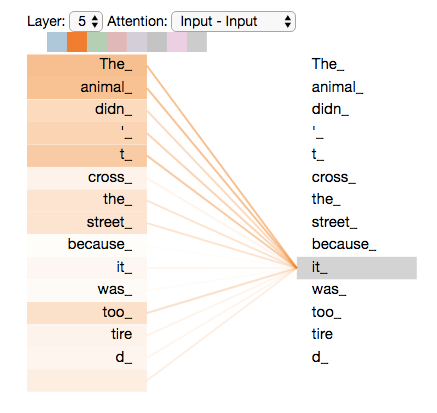
\includegraphics[width=10cm]{img/transformer_self-attention.png}
      \caption{Transformerにおけるself-attentionの仕組み、文献\cite{TheIllus32:online} より引用}
      \label{img:transformer_self-attention}
  \end{center}
\end{figure}

\subsection{BERT}
Transformerが発表された後に自然言語処理ではTransformerを用いた様々な発展モデルが発表された。そのうちのひとつがBidirectional Encoder Representations from \\Transformers(BERT)\cite{https://doi.org/10.48550/arxiv.1810.04805}である。BERTは、非常に大規模なTransformerのモデルを、文の一部をそれ以外の部分を使って予測することで、教師なしで学習(事前学習と呼ばれる)するというものである。これによって、言語の高レベルなニュアンスをエンコードできるようになる\cite{Sowmya_Vajjala2022-02-04}。
\begin{figure}[h]
  \begin{center}
      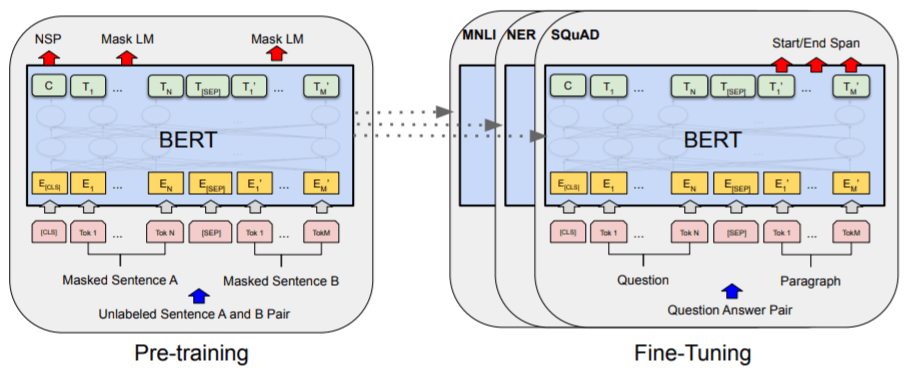
\includegraphics[width=10cm]{img/BERT-method.png}
      \caption{BERTの事前学習とファインチューニングされたタスクごとのモデル、文献\cite{https://doi.org/10.48550/arxiv.1810.04805} より引用}
      \label{img:BERT-method}
  \end{center}
\end{figure}
図\ref{img:BERT-method}の左側は事前学習されたモデルである。このモデルは、右側に示されているようなテキスト分類(MNLI)、固有表現認識(NER)、質問応答(SQuAD)のような自然言語処理タスクのためにファインチューニングを行う。事前学習された膨大な量の知識により、BERTは先述したようなさまざまなタスクのために知識を効率的に移転をすることができる。

%事前学習では、ラベルなしテキストデータを用いて、Next Sentence Prediction(NSP)と、
%TODO:時間あったらもっと詳しく書く

\subsection{SentenceBERT}
SentenceBERT\cite{arxiv.1908.10084}は文の埋め込み表現の構築のために改良を加えられたBERTである。事前学習済みBERTのBERTにPooling層を加え、自然言語推論タスクで追加学習を行うことで構築をされる。
類似文検索のタスクなどに用いられており、

\chapter{問題}
\label{issue}
% この研究が解く問題をシャープに記述する

本章では、サービス利用者がインターネットサービスを利用する際に利用規約を読む場面において、本研究の解決する問題について述べる。また、利用規約が読まれないことに対しての問題点や原因を明確化した後に、問題解決のための要件を述べる。

\section{利用規約の認知}
2020年に消費者庁が「デジタル・プラットフォーマーの取引慣行等に関する実態調査」の一環として、デジタル広告分野についての実態調査を行い、検索サービス及びSNSの利用者向け(消費者向け)アンケート調査を行った。この調査の結果を以下に示す。
\begin{figure}[h]
  \begin{center}
      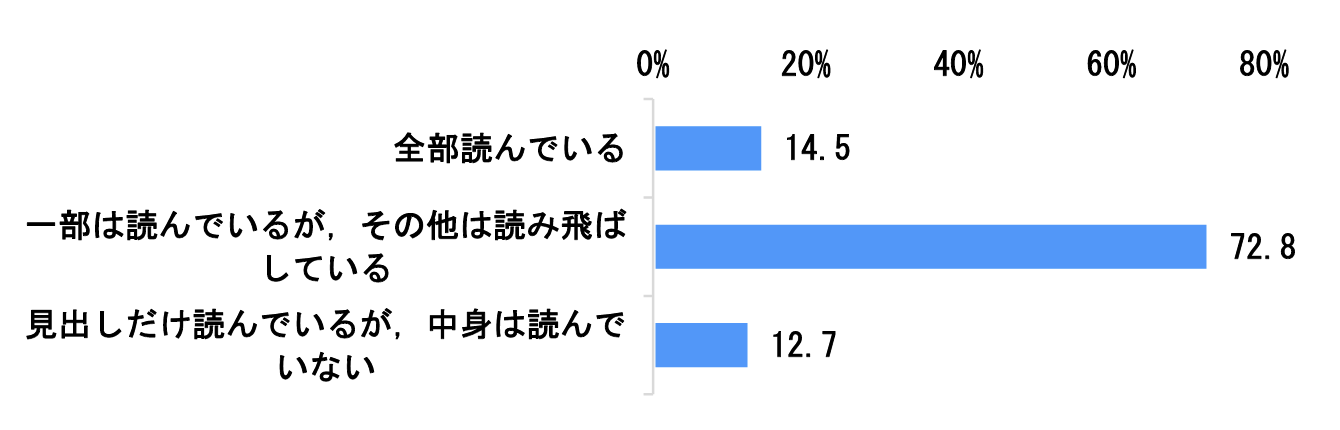
\includegraphics[width=13cm]{img/searchtosyomu.png}
      \caption{検索サービスの利用規約をどの程度読んでいるか(回答数:448)、文献\cite{jftc2021} より引用}
      \label{img:searcjtosyomu}
      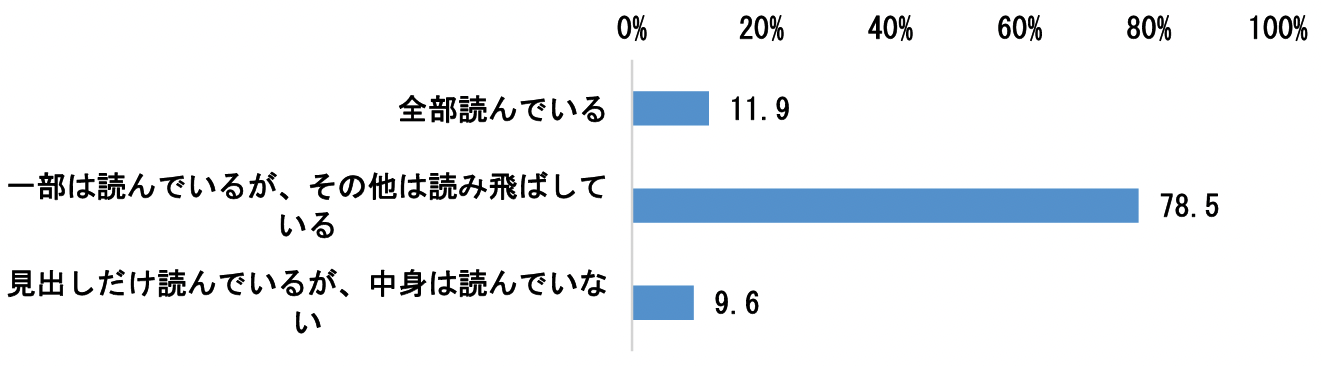
\includegraphics[width=13cm]{img/snstosyomu.png}
      \caption{SNS 等の利用規約をどの程度読んでいるか(回答数:929)、文献\cite{jftc2021} より引用}
      \label{img:snstosyomu}
  \end{center}
\end{figure}

図\ref{img:searcjtosyomu}、\ref{img:snstosyomu}では、それぞれ検索サービス、SNSについて「どの程度読んでいるか」についての調査が行われている。なお、この質問の前段では、「利用規約を認知しているか」についての質問があり、これについて「知っている」を選択した人がこの質問に回答している。このような調査では一般的に、社会適応バイアスにより高めの数値となってしまうことが多いが、それを指し引かなくとも、ほとんどの人が読み飛ばしているもしくは読んでいないという結果が示されている。

\begin{figure}[h]
  \begin{center}
      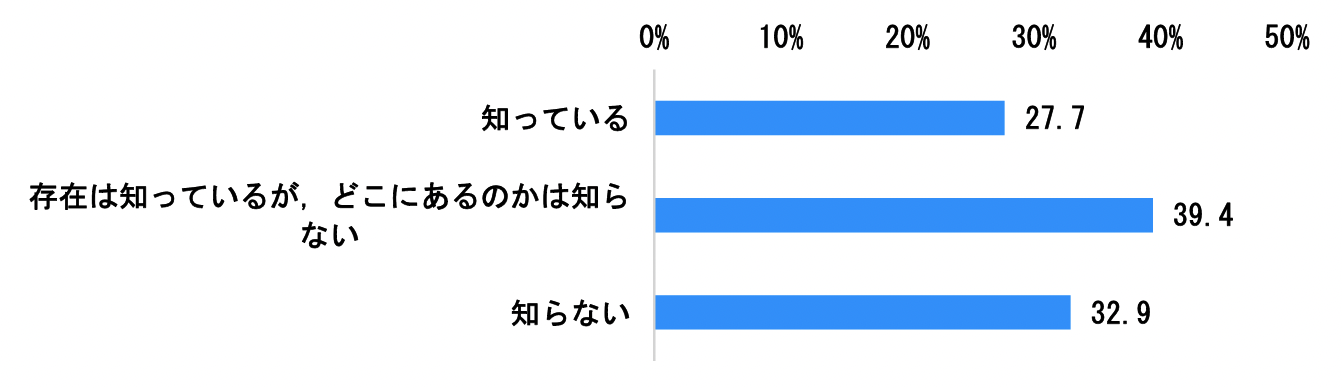
\includegraphics[width=13cm]{img/searchtosninchi.png}
      \caption{検索サービスの利用規約の認知(回答数:2,000)、文献\cite{jftc2021} より引用}
      \label{img:searchtosninchi}
      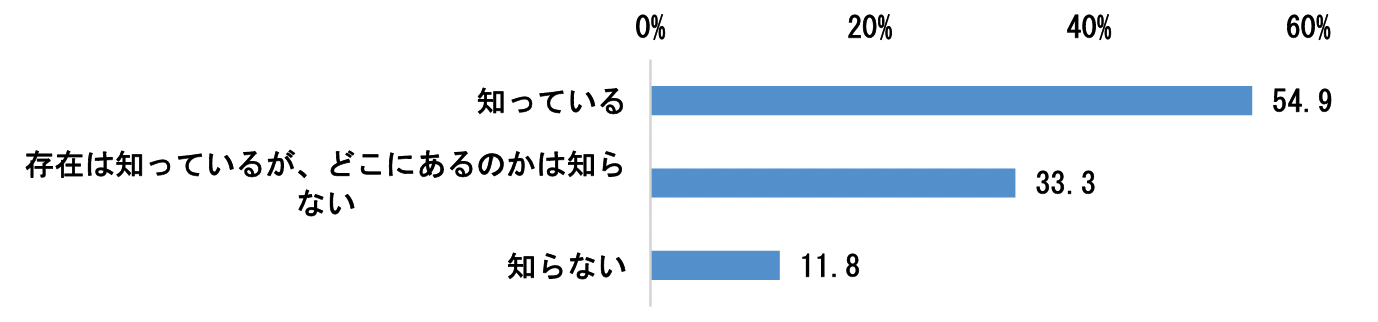
\includegraphics[width=13cm]{img/snstosninchi.png}
      \caption{SNS 等の利用規約の認知(回答数:2,000)、文献\cite{jftc2021}  より引用}
      \label{img:snstosninchi}
  \end{center}
\end{figure}

本研究では、「利用規約の認知」についてはアプローチが非常に困難であることから、この認知を前提として、「利用規約を読み飛ばしてしまう」事象を問題として定義し、それに対するアプローチについての検討を行う。

\section{利用規約の読解}
オムリ・ベン=シャハーほか(2022)\cite{sonokiyaku2022}は、利用規約をはじめとして、食品表示ラベル、著作権表示警告、金融機関の取引前リスク告知、医療行為の場面で行われるインフォームドコンセントなど、法令などで規制されている同意を求める行為をまとめて「開示主義」と定義し、これらの規制を「義務的情報開示」と定義している。その中で、開示主義が失敗していると述べている。(要追記)

\section{問題の定義}
先述したように、利用規約が読まれていないという問題がある。このことは、インターネット上でのサービスを利用する際に、利用規約に関して十分な理解を持っていないままサービスの利用を開始してしまうことになる。これにより、将来的に問題が発生する可能性を孕んだまま利用を継続することになる。この理由の1つとして、利用規約を集中して読むために必要な時間が長すぎる点が挙げられる。本研究では、そのようなユーザーに利用規約を読むことができるように利用規約の読解時間に要する時間が長いということを問題定義とする。

%\section{問題解決の要件}

\chapter{仮説}
\label{proposed}
%どうやったら解けると考えているか (検証可能なように書く)

本章では仮説について述べる。

\section{概要}
本研究では、利用規約の読解支援のために、利用規約の読解時間を短縮すること


%%% Local Variables:
%%% mode: japanese-latex
%%% TeX-master: "../bthesis"
%%% End:

\chapter{実験}
\label{experiment}
%仮説を検証するためにやったことを再現可能な様に書く
%結果も書く

本章では提案手法の実装について述べる。

\section{概要}
\label{sub:実験概要}
本研究の仮説をもとに、システムの実装をおこなった。
\begin{figure}[h]
  \begin{center}
      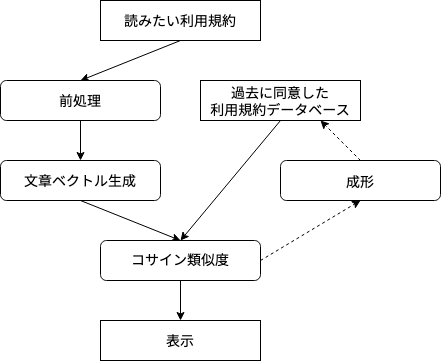
\includegraphics[width=10cm]{img/system.drawio.png}
      \caption{類似条文検出の実装イメージ}
      \label{img:類似条文検出の実装イメージ}
  \end{center}
\end{figure}
図\ref{img:類似条文検出の実装イメージ}に示したように、まず、読みたい利用規約について、前処理を行う。ここでは、URLの置き換え、かっこなどの記号の除去、「利用者」「会員」などを「ユーザー」に表現を揃えるなどの処理を行う。また、条文と条文でない部分(「第○条」、「以上」のような表現など)を除去するための情報がここで与えられる。本研究では、条文でない部分に関しての情報はあらかじめ手作業で与えることとした。その後、文章ベクトルを生成する。本研究では、東北大乾研の大規模日本語モデルを利用した。そして、生成された文章ベクトルと過去に同意した利用規約データベースに保存されている文ベクトルとコサイン類似度の計算を行い、表示する。表示したのち、利用者が同意をした場合は、文章の成形、保存された文章に前処理で取り除けなかった余分な情報などが含まれないかを確認し、必要であれば編集と文章ベクトルの再生成を行い、過去に同意した利用規約データベースに保存する。その情報が増えることにより、検出される条文が増える。同意しなかった場合は保存をしない。

\section{表示方法}
表示方法については、利用規約の類似条文検出に加えて、判断の材料にするために、類似度の高い順に3つの条文とその条文をもつサービス名、コサイン類似度を表示した。3つに設定した根拠としては、他サービスの条文と比較するときに複数サービスの条文と比較することで、より類似度を利用者が比較しやすいと考えたからである。

%\section{実行環境}
%\begin{center}
%  \begin{tabular}{ll} \hline
%    項目 & 仕様 \\ \hline \hline
%    環境 & Azure Web App Service\\
%    インスタンス & B1 \\
%    コア数 & 1 \\
%    RAM & 1.75GB \\ \hline
%  \end{tabular}
% \end{center}

%%% Local Variables:
%%% mode: japanese-latex
%%% TeX-master: "../bthesis"
%%% End:

\chapter{評価}
\label{discussion}
%結果を解釈・評価する
本章では、\ref{experiment}章で行った実装のの評価について述べる。

\section{評価内容}
評価として、以下の内容を検証する。まず、評価を行うために利用規約を準備する。その利用規約に関するクイズを用意し、実際に利用をしてもらい、読解時間を短縮できるかについて検証を行う。また、クイズを用いて通常の利用規約の表示と提案システムの表示を比較し、理解度の測定を行う。
%実装が実際に利用できるという観点から、1つ目は類似度の計算が一般的な利用に問題ない時間であるかを測定する。

\section{評価のための利用規約}
\label{sec:評価のための利用規約}
提案手法の評価のために、利用規約をAlpha社、Beta社、Gamma社、Delta社、Epsilon社、Zeta社、Eta社の8つ用意した。これらは、実在する会社やサービスの利用規約を実験用に会社名やサービス名を置き換えたり、一部条項の書き換えをおこなったものである。また、評価で利用規約の読解に要した時間を測定するために、条文の数を揃える作業を行なっている。利用規約については、以下のような観点から選んだ。
\begin{itemize}
  \item 特定のサービスの専門的な用語ばかりではない
  \item 条文数が極端に多くない
  \item 可能な限り違う種類のサービスを展開している
\end{itemize}
これらの条件から、実在する利用規約の選定を行い、これらについて社名の変更などや、読解時間が条文数に影響されてしまうことが考えられるため、通常の状態で読解時間が同じになるように条文の編集などを行なった。

\begin{table}[h]
  \centering
  \caption{実験用利用規約の一覧}
  \begin{tabular}{cc}
  \hline
  実験用社名    & 主に元にした利用規約\\ \hline\hline
  Alpha社   & 掲示版・SNS系向きの利用規約の雛形(ひな型)\tablefootnote{https://kiyaku.jp/hinagata/sns.html}\\ \hline\
  Beta社    & Annict\tablefootnote{https://annict.com/terms}\\ \hline\
  Gamma社   & 鎌倉新書\tablefootnote{https://www.kamakura-net.co.jp/servicepolicy/}\\ \hline\
  Delta社   & クックパッド\tablefootnote{https://cookpad.com/terms/free}\\ \hline\
  Epsilon社 & 第一法規\tablefootnote{https://www.daiichihoki.co.jp/support/rules/}\\ \hline\
  Zeta社    & IRIAM\tablefootnote{https://www.live.iriam.com/terms}\\ \hline\
  Eta社     & 三越伊勢丹WEB会員規約\tablefootnote{https://www.mistore.jp/shopping/help/guide/terms\_h.html}\\ \hline\
  Theta社   & Z会ソリューションズ\tablefootnote{https://www.zkai.co.jp/assess/terms}\\ \hline
  \end{tabular}
\end{table}
評価の際はこれらの実験用社名については被験者にわかるように明示をしている。

\section{評価のためのクイズ}
\label{sec:評価のためのクイズ}
本提案手法により通常の利用規約を読んだときよりも著しく利用者の理解度が下がっていると、本提案手法は読解の阻害になってしまうと考えられるため、そのようなことが起きていないかを確認するために、クイズを設定した。クイズに内容は、評価のための利用規約の中から広く選び、また、一部書き換えた条文などをクイズとして出題をした。問題数は各利用規約について2択のクイズを2問となっている。問題間での正答率の差を見るために、問題に難易度の差を意図的につけた。これにより、低難易度の問題は正答率がどちらも高くなければいけなく、高難易度の場合は正答率に差が出るかを検証できる。

\section{評価用実験システムの環境}
\label{sec:評価用実験システムの環境}
本提案システムが有効に機能するかを実験するために、評価用のシステムを構築した。容易に実験が可能なように、PythonのフレームワークであるFlaskでWebサイトとして提案システムが容易に扱えるようにした。そのシステムをAzure Web App Service上に展開をし、そこへのアクセスをもって実験を行えるようにした。

一般的なインターネットユーザーを想定し、かつ、利用規約を読んだことがあるという観点から、クラウドソーシングサービスである、クラウドワークス\footnote{https://crowdworks.jp/}を用いて被験者を募った。クラウドワークスの利用者は、登録時にクラウドワークスの利用規約を読んだことがあるので、利用規約を読まなければいけないという経験がある被験者の集団を作ることができる。なお、報酬は、1人あたり100円とした。被験者には、初めにページにて本提案手法の趣旨の説明を行なった。
\begin{figure}[h]
  \begin{center}
      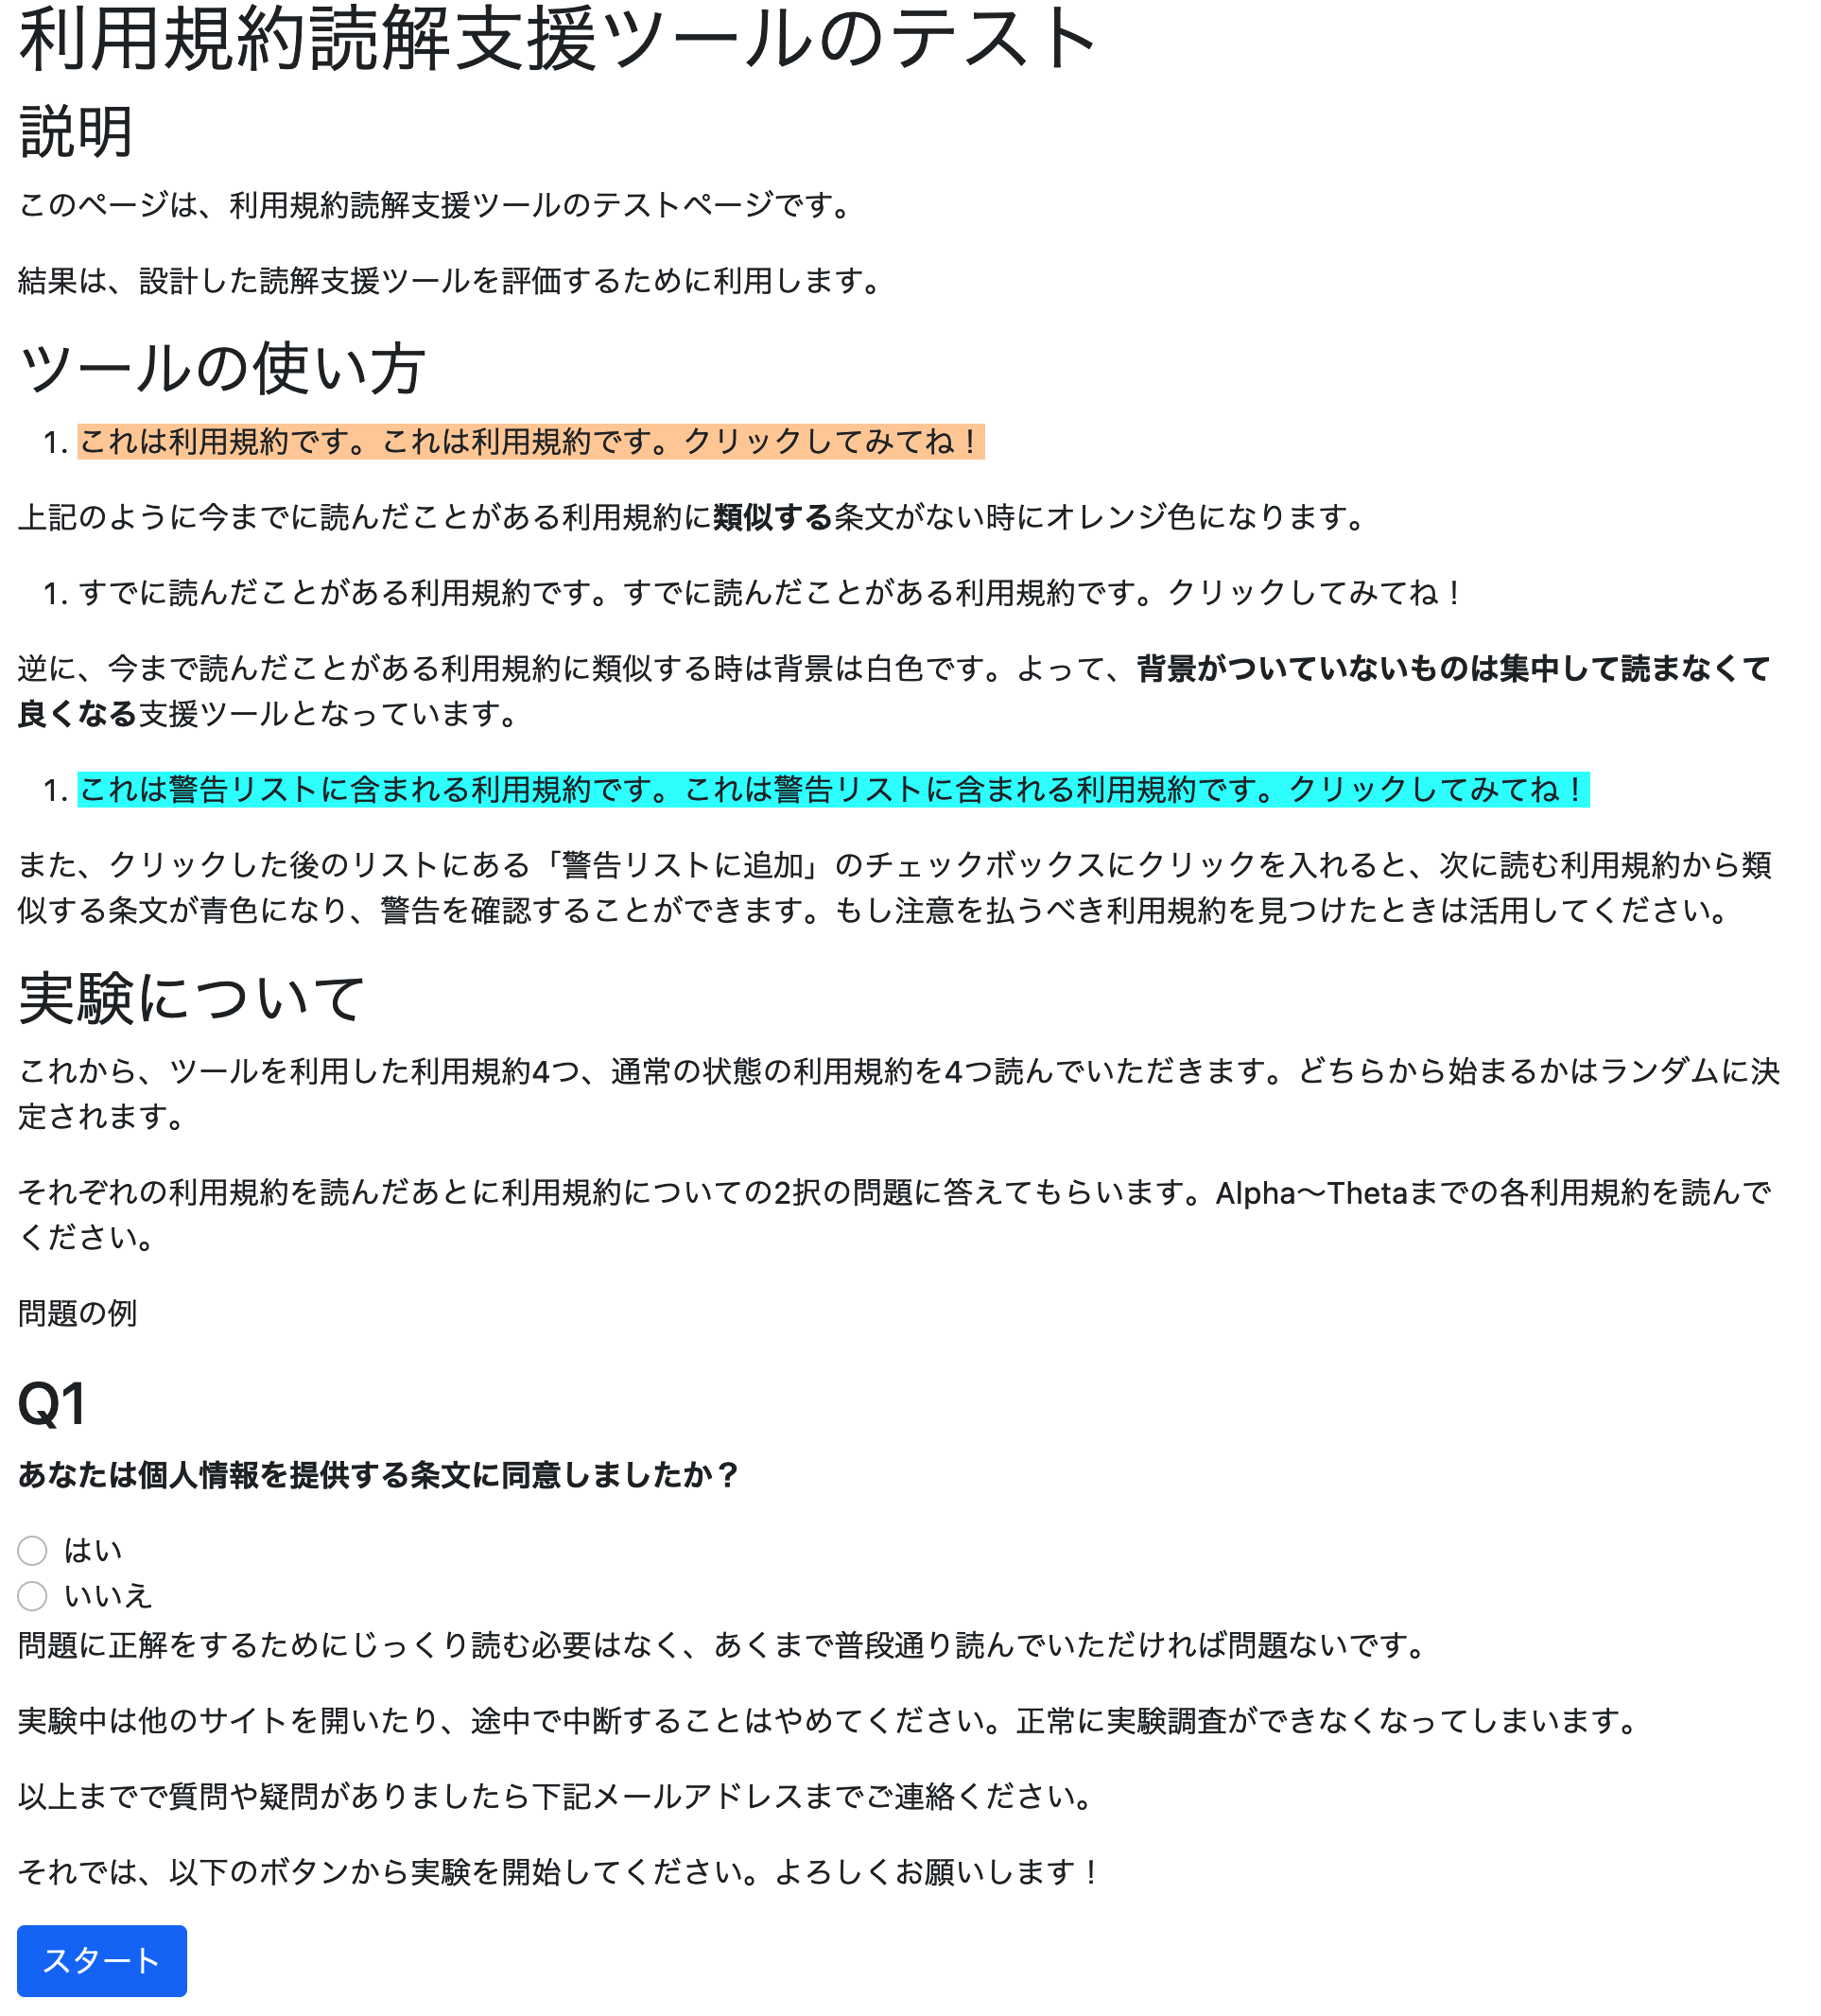
\includegraphics[width=16cm]{img/teststart1.png}
      \caption{実験概要説明ページ}
      \label{img:実験概要説明ページ}
  \end{center}
\end{figure}
被験者への説明は、「利用規約を読みやすくするためのツールのテスト」であるという表現にとどめ、本来の目的である、利用規約の読解時間短縮ということは伝えていない。これは、本来の実験の目的を最初に伝えてしまうと、被験者の読解時間の変動が起きてしまうと考えられるからである。

被験者は説明を読んだ後、利用規約を8つ読んでいく。提案システムとシステムを通さない通常の利用規約表示を比較するため、順番はランダムでかつ4つずつを読む形にした。8つの利用規約の順番もランダムであり、ランダムでどのような順序で実験が行われるかは予め被験者に通知をした。利用規約を読む時間をそれぞれ環境を作成した。また、追加実験として、8つの利用規約全てに提案システムを適用した場合の実験も行なった。
\begin{figure}[h]
  \begin{center}
      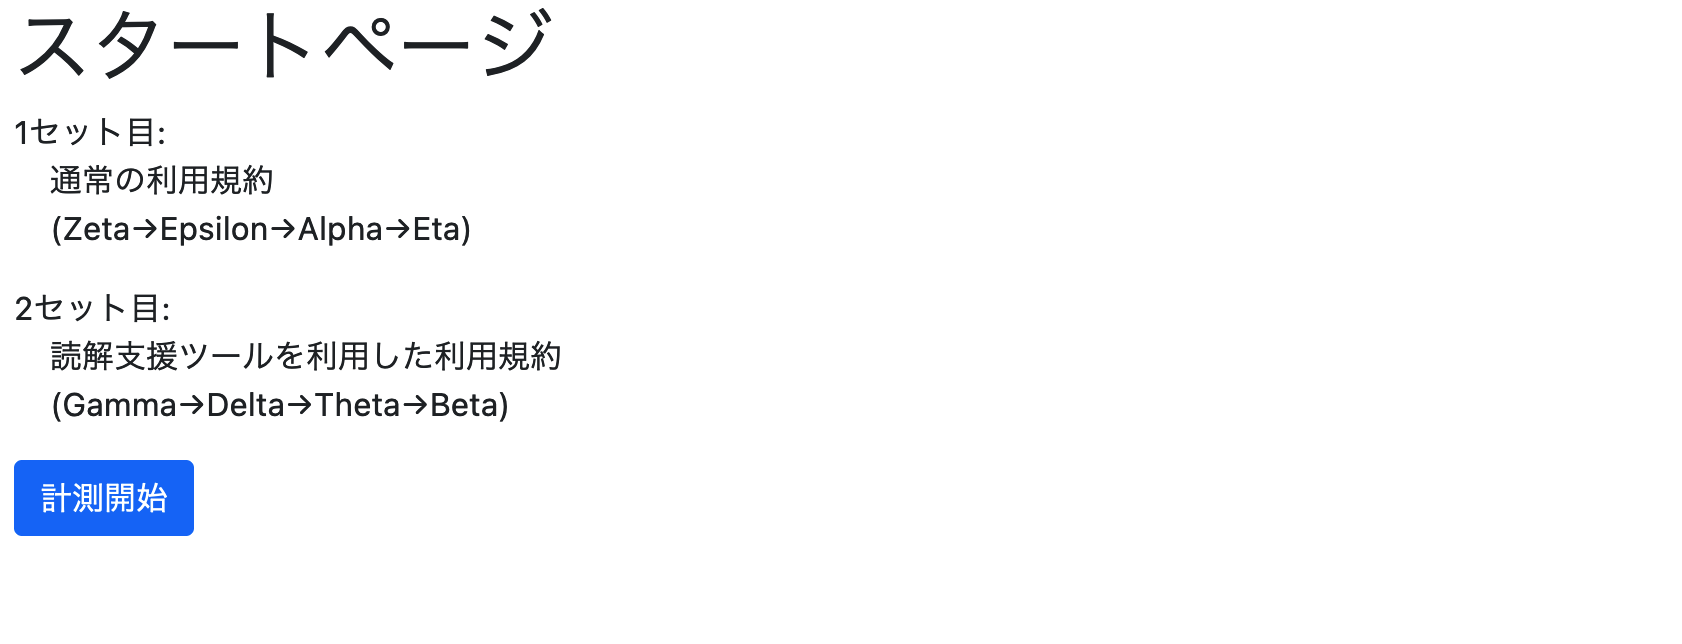
\includegraphics[width=16cm]{img/teststart2.png}
      \caption{実験順序説明ページ}
      \label{img:実験順序説明ページ}
  \end{center}
\end{figure}

そのあとは利用規約を表示し、「同意する」「同意しない」をクリックする。その後、\ref{sec:評価のためのクイズ}節で示したクイズが表示される。クイズに回答した後は次の利用規約を表示する表示が繰り返され、全ての利用規約を閲覧し終わったあとはアンケートに回答を依頼した。

\section{結果}
\ref{sec:評価用実験システムの環境}節の実験を行なった結果を示す。なお、クラウドワークス上での回答が不十分であったり、途中で実験ページから離れてしまった場合など、正常にデータを取得できなかった場合を予め除外した。通常の状態で4つ、提案システムで4つ閲覧するパターンは127件、提案システムで8つ閲覧するパターンは35件のデータを得ることができた。

\subsection{読解時間}
本提案システムは、利用規約を読んでいくごとに注目するべき部分が減ることで読解時間が減るという趣旨であるため、複数回利用規約を読む必要がある。今回の評価用実験システムは被験者の負担を考え、利用規約を4つずつ読み、読解時間を計測した。よって、通常表示の利用規約と提案システムを利用して読解した4回目を比較した。
\begin{figure}[h]
  \begin{center}
      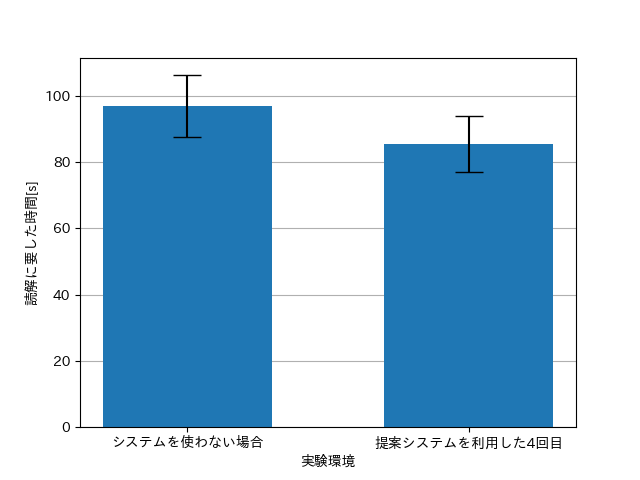
\includegraphics[width=13cm]{img/tgraph4.png}
      \caption{通常の表示の平均時間と提案システムの4回目の読解時間の比較/標準誤差}
      \label{img:通常の表示の平均時間と提案システムの4回目の読解時間の比較/標準誤差}
  \end{center}
\end{figure}
\begin{table}[h]
  \caption{通常の表示の平均時間と提案システムの4回目の読解時間}
  \label{tab:通常の表示の平均時間と提案システムの4回目の読解時間}
  \centering
  \begin{tabular}{ccc}
    \hline
    値[s]  & 通常の表示の平均時間  &  提案システムの4回目の読解時間  \\
    \hline \hline
    平均値  & 96.87  & 85.31 \\
    中央値  & 57.97   & 49.71 \\
    標準偏差  & 104.65  & 95.36 \\
    分散  &  10950.64  &  9093.15 \\
    標準誤差  &  9.29  &  8.46 \\
    \hline
  \end{tabular}
\end{table}
図\ref{img:通常の表示の平均時間と提案システムの4回目の読解時間の比較/標準誤差}、表\ref{tab:通常の表示の平均時間と提案システムの4回目の読解時間}という結果となった。対応のあるt検定で片側検定を行い、「提案システムの4回目の読解時間は通常の表示の平均時間よりも短い」という仮説を検証した結果、$p=0.03<0.05$となり、有意水準5\%でこの仮説が正しいことが示された。

また、本提案システムは利用規約を読解した量を増やしていくとさらに注目するべき部分が減っていき、さらに読むべき部分が減ると考えられる。8つ全ての利用規約を読解した場合とも比較を行う。本実験は、別の集団のため、対応がないことに留意する必要がある。
\begin{figure}[h]
  \begin{center}
      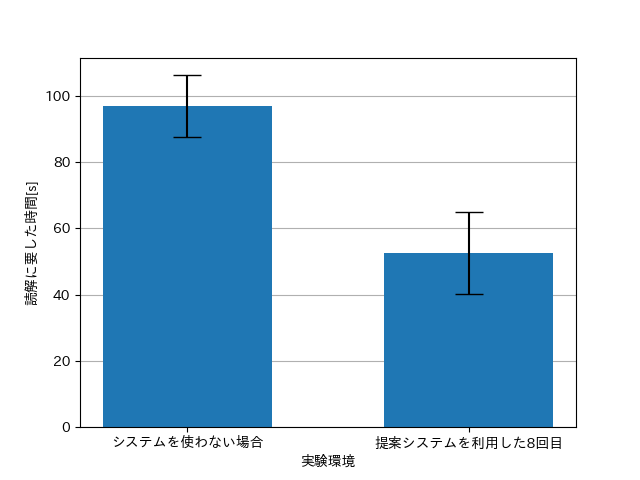
\includegraphics[width=13cm]{img/tgraph8.png}
      \caption{通常の表示の平均時間と提案システムの8回目の読解時間の比較/標準誤差}
      \label{img:通常の表示の平均時間と提案システムの8回目の読解時間の比較/標準誤差}
  \end{center}
\end{figure}
\begin{table}[h]
  \caption{提案システムの8回目の読解時間}
  \label{tab:提案システムの8回目の読解時間}
  \centering
  \begin{tabular}{ccc}
    \hline
    値[s]  & 提案システムの8回目の読解時間  \\
    \hline \hline
    平均値  & 52.50 \\
    中央値  & 28.57 \\
    標準偏差  & 72.68 \\
    分散  &  5282.13 \\
    標準誤差  & 12.28 \\
    \hline
  \end{tabular}
\end{table}
図\ref{img:通常の表示の平均時間と提案システムの8回目の読解時間の比較/標準誤差}、表\ref{tab:提案システムの8回目の読解時間}という結果になった。対応のないt検定で片側検定を行い、「提案システムの8回目を読んだ集団の読解時間は通常の表示を読んだ集団の平均読解時間よりも短い」という仮説を検証した結果、$p=0.01<0.05$となり、有意水準5\%でこの仮説が正しいことが示された。

\subsection{理解度}
提案システムを通して利用規約を読解したとき、通常の利用規約表示よりも理解度が落ちていないことを、クイズの正答率をもとに評価を行う。通常の表示を4つ、提案システムで4つ読んだ集団の正答率それぞれを比較する。
\begin{figure}[h]
  \begin{center}
      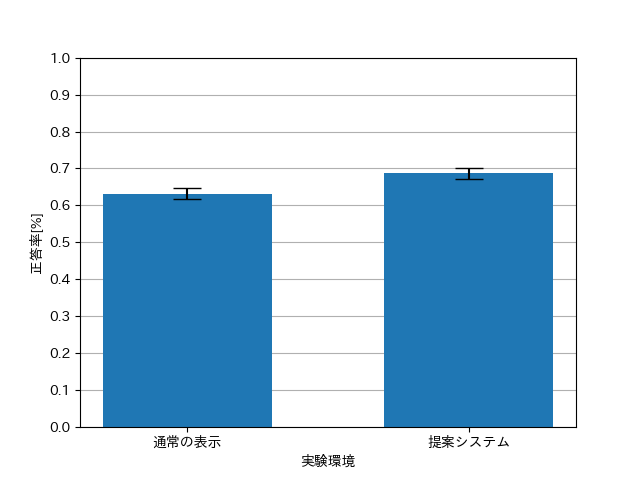
\includegraphics[width=13cm]{img/answerne4.png}
      \caption{通常の表示と提案システムの正答率の比較/標準誤差}
      \label{img:通常の表示と提案システムの正答率の比較/標準誤差}
  \end{center}
\end{figure}
\begin{table}[h]
  \caption{通常の表示と提案システムの正答率}
  \label{tab:通常の表示と提案システムの正答率}
  \centering
  \begin{tabular}{ccc}
    \hline
    正答率[\%]  & 通常の表示  &  提案システム  \\
    \hline \hline
    平均値  & 0.63  & 0.69 \\
    中央値  & 0.63   & 0.75 \\
    標準偏差  & 0.18  & 0.18 \\
    分散  &  0.03  &  0.03 \\
    標準誤差  &  0.02  &  0.02 \\
    \hline
  \end{tabular}
\end{table}
図\ref{img:通常の表示と提案システムの正答率の比較/標準誤差}、表\ref{tab:通常の表示と提案システムの正答率}という結果となった。対応のないt検定で片側検定を行い、「通常の表示よりも提案システムの正答率の方が高い」という仮説を検証した結果、$p<0.01$となり、有意水準1\%でこの仮説が正しいことが示された。また、問題ごとの正答率について個別に比較を行ったが、ほとんどの場合が提案システムの方が正答率が高かった。一部、正答率が低い場合があったが、数\%であり、検定をしても有意差は見られないため、誤差の範囲であるといえ、先述した著しく理解度が落ちていない証明ができた。

以下に、各問題についての正答率のグラフを示す。
\begin{figure}[h]
  \begin{center}
      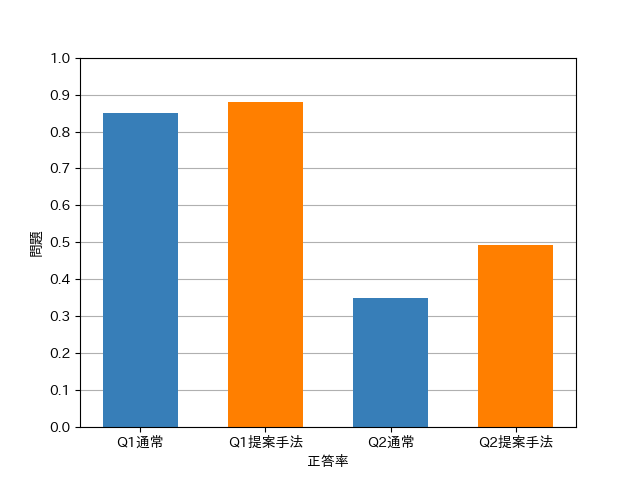
\includegraphics[width=13cm]{img/qgraphAlpha.png}
      \caption{Alpha社クイズの正答率}
      \label{img:Alpha社クイズの正答率}
  \end{center}
\end{figure}
\begin{figure}[h]
  \begin{center}
      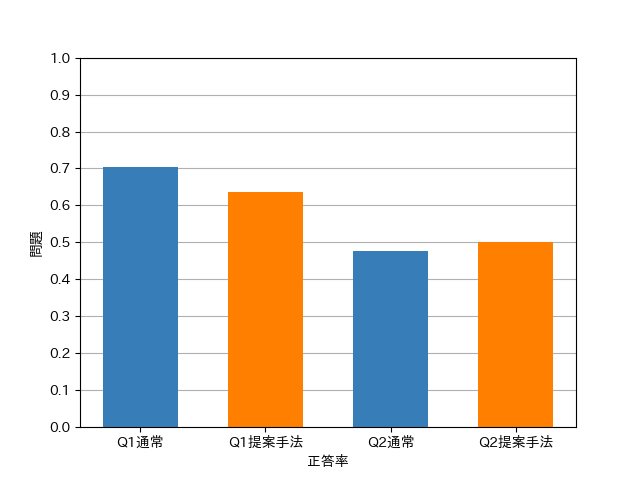
\includegraphics[width=13cm]{img/qgraphBeta.png}
      \caption{Beta社クイズの正答率}
      \label{img:Beta社クイズの正答率}
  \end{center}
\end{figure}
\begin{figure}[h]
  \begin{center}
      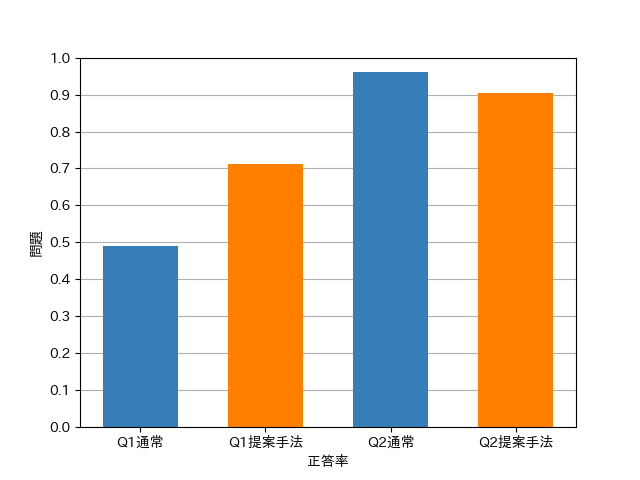
\includegraphics[width=13cm]{img/qgraphGamma.png}
      \caption{Gamma社クイズの正答率}
      \label{img:Gamma社クイズの正答率}
  \end{center}
\end{figure}
\begin{figure}[h]
  \begin{center}
      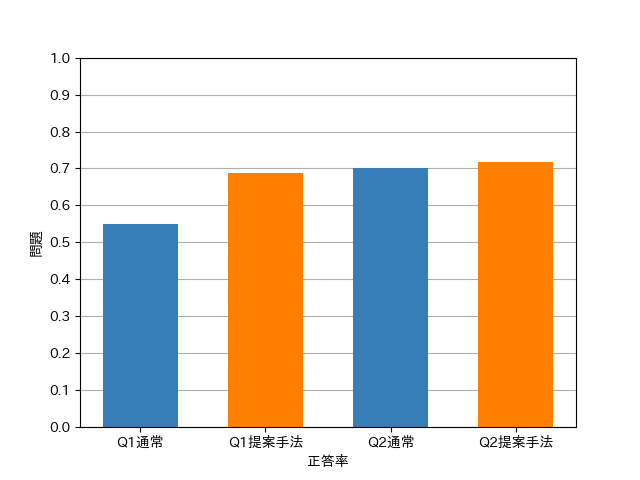
\includegraphics[width=13cm]{img/qgraphDelta.png}
      \caption{Delta社クイズの正答率}
      \label{img:Delta社クイズの正答率}
  \end{center}
\end{figure}
\begin{figure}[h]
  \begin{center}
      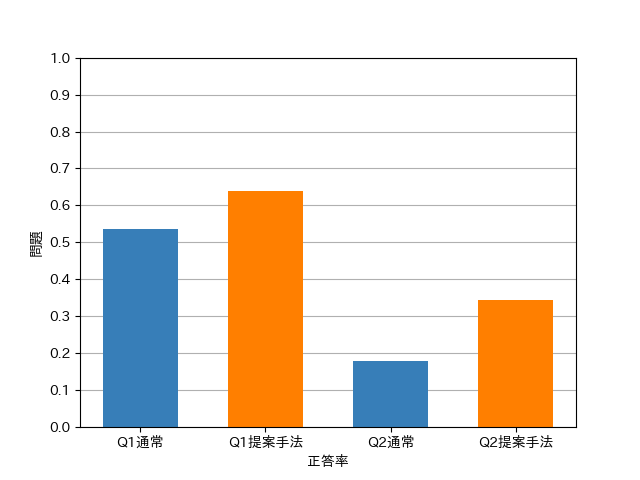
\includegraphics[width=13cm]{img/qgraphEpsilon.png}
      \caption{Epsilon社クイズの正答率}
      \label{img:Epsilon社クイズの正答率}
  \end{center}
\end{figure}
\begin{figure}[h]
  \begin{center}
      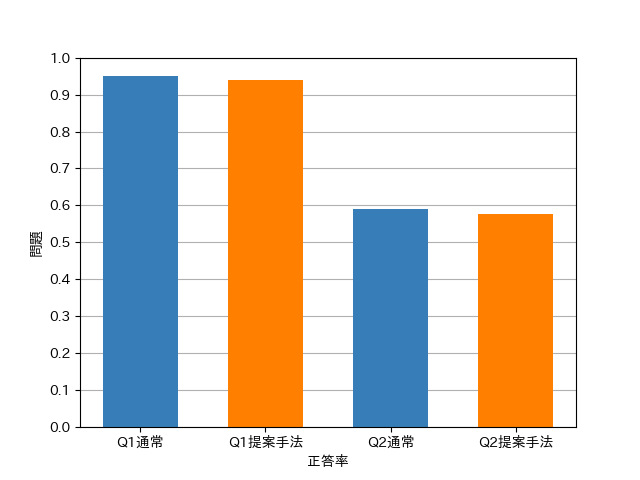
\includegraphics[width=13cm]{img/qgraphZeta.png}
      \caption{Zeta社クイズの正答率}
      \label{img:Zeta社クイズの正答率}
  \end{center}
\end{figure}
\begin{figure}[h]
  \begin{center}
      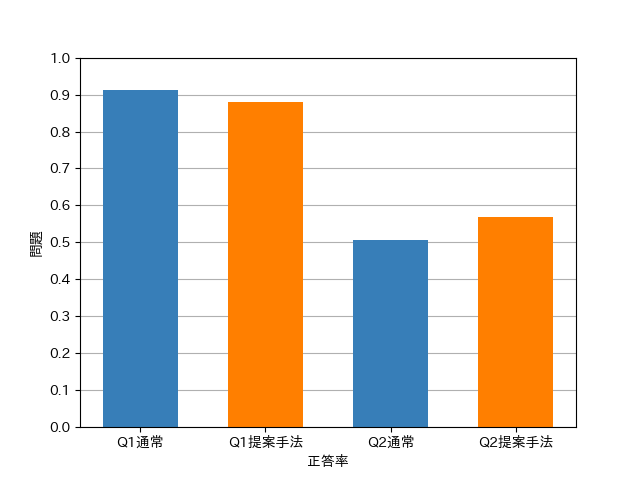
\includegraphics[width=13cm]{img/qgraphEta.png}
      \caption{Eta社クイズの正答率}
      \label{img:Eta社クイズの正答率}
  \end{center}
\end{figure}
\begin{figure}[h]
  \begin{center}
      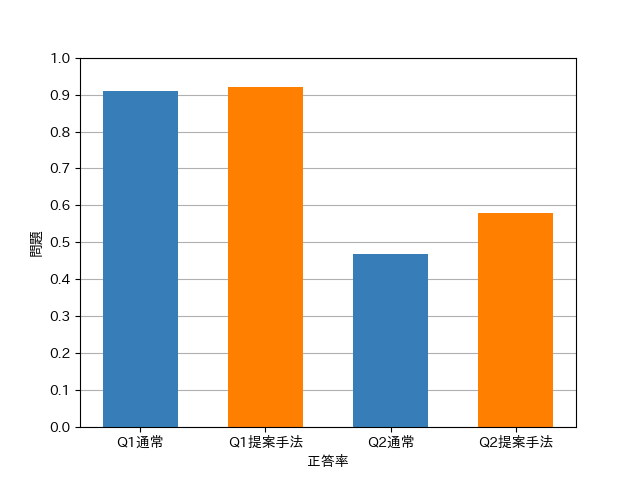
\includegraphics[width=13cm]{img/qgraphTheta.png}
      \caption{Theta社クイズの正答率}
      \label{img:Theta社クイズの正答率}
  \end{center}
\end{figure}

%%% Local Variables:
%%% mode: japanese-latex
%%% TeX-master: "./thesis"
%%% End:

\chapter{関連研究}
\label{related}
%他人の先行研究・事例で、自分の研究が戦う相手について述べて比較する

本章では、本研究の関連研究を示す。

\section{機械学習を用いた利用規約からの未知条項の抽出に関する研究(中村ら 2018)}

\section{CLAUDETTE: an automated detector of potentially unfair clauses in online terms of service(Lippiら 2019)}
CLAUDETTEは、

\section{利用規約中の不公平文の自動検出(青山ら 2019)}

\section{力約: ソフトウェアインストール時における利用規約に応じた力覚提示デバイスの開発(豊島ら 2015)\cite{weko_145305_1}}
力約\cite{weko_145305_1}は、利用規約に同意する際の「同意し契約を交わそうとしている内容の重大さ」に着目し、その重大さをユーザーに伝えるための図\ref{img:rikiyaku}に示すボタン型デバイスを提案している。利用規約を読み飛ばしてしまうという事象を、利用規約の読解の後の同意を押すタイミングでデバイスを利用し、規約内容に応じて「力覚」に作用させることで、より内容の重大さを訴えかけることを試みている。この研究は、同意の重大さを利用者が感じ取ることの困難性を示しており、利用規約の同意ボタンを物理的かつ内容による必要な力の強さの調整を試みている。本研究では、利用規約の重大さについて、ハイライトを持ってより注目を促すように作用をさせている。そのことにより、より条文の内容を読み込むように促せていると考えられる。
\begin{figure}[h]
  \begin{center}
      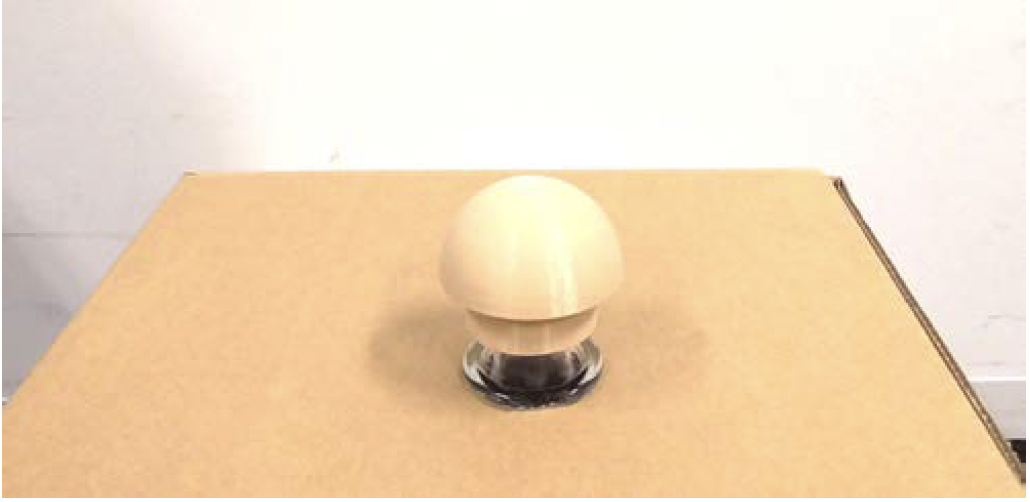
\includegraphics[width=13cm]{img/rikiyaku.png}
      \caption{力約ボタンの外観、文献\cite{weko_145305_1} より引用}
      \label{img:rikiyaku}
  \end{center}
\end{figure}

%%% Local Variables:
%%% mode: japanese-latex
%%% TeX-master: "../thesis"
%%% End:

\chapter{結論}
\label{conclusion}
%まとめる、次に続く研究への課題を書く、自分のメッセージを書く

本章では,本研究のまとめと今後の課題を示す.

\section{本研究のまとめ}

\section{本研究の課題}
本節では、本研究で提案したシステムの課題と展望について述べる。

\subsection{構想}
本研究の提案をより、社会実装しやすくするためのものとして、利用規約図書館のような構想がある。この構想は筆者の卒業論文で提案されている利用規約をユーザー同士でとりまとめて保存しておくシステムである。このような仕組みを構築することで、同じ約款を大量の人が同意する点に着目し、以下のようなメリットが考えられる。
\begin{enumerate}
  \item 利用規約の変更などを利用者同士で確認し、追従することができる。
  \item 本研究の実装の自然言語処理などの手順を誰か1人が取ることで、その成果を他の利用者も利用することができる。
\end{enumerate}
本研究では特に、文ベクトルの生成に利用者の計算リソースを消費してしまうという課題があり、さらに、文量が非常に多い約款の場合はシステムの利用のための時間がかかってしまうため、この仕組みをもとにシステムを稼働することができれば、より利用しやすいシステムになると考えられる。しかし、この提案にも維持者や管理人が必要になるために、このコストを誰が負担するかという問題がある。論文では、この問題を克服するために、適格消費者団体のような、現在利用規約の監視や裁判を消費者側の立場で行なっている団体が管理することを提案している。 


%%% Local Variables:
%%% mode: japanese-latex
%%% TeX-master: "../thesis"
%%% End:

%\appendix
\chapter{実験に利用した利用規約}
実験に利用した利用規約を以下に示す。なお、利用した利用規約は実在する利用規約をベースに社名やサービス名などを置き換え、実験用に条項の一部を変更したものである。

\section{Alpha社}

%\chapter*{謝辞}
\addcontentsline{toc}{chapter}{謝辞}
\label{thanks}

謝辞



%%% Local Variables:
%%% mode: japanese-latex
%%% TeX-master: "../yummy_bthesis"
%%% End:


\renewcommand{\thechapter}{\Alph{chapter}}
\setcounter{chapter}{0}
\vspace{-5mm}


\bibliographystyle{unsrt}\pagestyle{plain}
\bibliography{./bib/cites}\pagestyle{plain}
\thispagestyle{plain}%bibtex


\end{document}

%%% Local Variables:
%%% mode: japanese-latex
%%% TeX-master: t
%%% End:
